\usetikzlibrary{shapes.geometric}
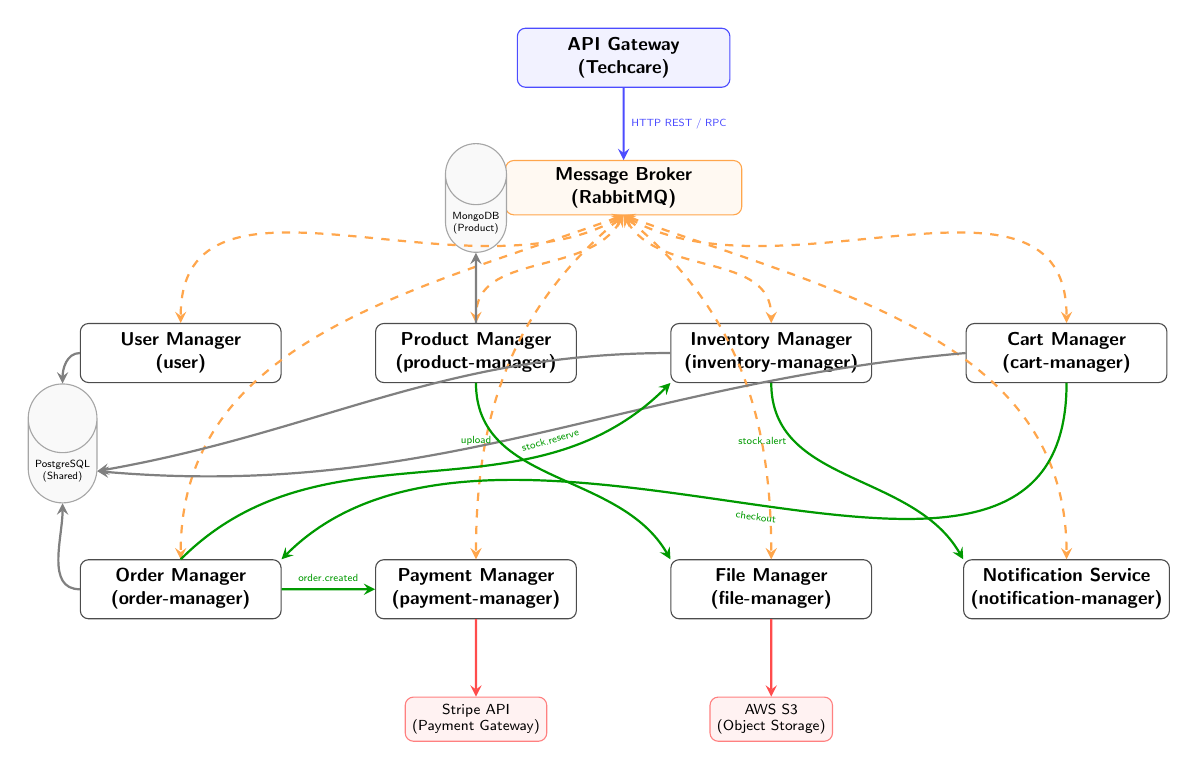
\begin{tikzpicture}[
    scale=0.75,
    transform shape,
    service/.style={
        draw=black!70,
        fill=white,
        minimum width=3.4cm,
        minimum height=1.0cm,
        align=center,
        font=\small\sffamily\bfseries,
        rounded corners=3pt
    },
    gateway/.style={
        draw=blue!70,
        fill=blue!5,
        minimum width=3.6cm,
        minimum height=1.0cm,
        align=center,
        font=\small\sffamily\bfseries,
        rounded corners=3pt
    },
    db/.style={
        cylinder,
        draw=gray!70,
        fill=gray!5,
        shape border rotate=90,
        minimum width=1.0cm,
        minimum height=1.2cm,
        font=\tiny\sffamily,
        align=center
    },
    broker/.style={
        draw=orange!70,
        fill=orange!5,
        minimum width=4.0cm,
        minimum height=0.8cm,
        align=center,
        font=\small\sffamily\bfseries,
        rounded corners=3pt
    }
]

    % ==========================================
    % NODES PLACEMENT
    % ==========================================

    % Gateway (Top Center)
    \node[gateway] (Gateway) at (0.0, 4.0) {API Gateway\\(Techcare)};

    % Broker RabbitMQ (Middle Center, between Gateway and Services)
    \node[broker] (RabbitMQ) at (0.0, 1.8) {Message Broker\\(RabbitMQ)};

    % ROW 1: Upper Services
    \node[service] (UserSvc) at (-7.5, -1.0) {User Manager\\(user)};
    \node[service] (ProductSvc) at (-2.5, -1.0) {Product Manager\\(product-manager)};
    \node[service] (InventorySvc) at (2.5, -1.0) {Inventory Manager\\(inventory-manager)};
    \node[service] (CartSvc) at (7.5, -1.0) {Cart Manager\\(cart-manager)};

    % ROW 2: Lower Services
    \node[service] (OrderSvc) at (-7.5, -5.0) {Order Manager\\(order-manager)};
    \node[service] (PaymentSvc) at (-2.5, -5.0) {Payment Manager\\(payment-manager)};
    \node[service] (FileSvc) at (2.5, -5.0) {File Manager\\(file-manager)};
    \node[service] (NotificationSvc) at (7.5, -5.0) {Notification Service\\(notification-manager)};

    % Databases
    \node[db] (PostgresDB) at (-9.5, -3.0) {PostgreSQL\\(Shared)};
    \node[db] (MongoDB) at (-2.5, 1.2) {MongoDB\\(Product)};

    % External Services
    \node[draw=red!50, fill=red!5, rounded corners=3pt, font=\scriptsize\sffamily, align=center, minimum width=2.0cm] (Stripe) at (-2.5, -7.2) {Stripe API\\(Payment Gateway)};
    \node[draw=red!50, fill=red!5, rounded corners=3pt, font=\scriptsize\sffamily, align=center, minimum width=2.0cm] (S3) at (2.5, -7.2) {AWS S3\\(Object Storage)};

    % ==========================================
    % CONNECTIONS
    % ==========================================

    % Gateway to RabbitMQ (HTTP to RPC/RabbitMQ)
    \draw[->, >=stealth, thick, blue!70] (Gateway) -- (RabbitMQ) node[midway, right, font=\tiny\sffamily] {HTTP REST / RPC};

    % RabbitMQ to Services
    \draw[dashed, <->, >=stealth, thick, orange!70] (RabbitMQ.south) to[out=210, in=90] (UserSvc.north);
    \draw[dashed, <->, >=stealth, thick, orange!70] (RabbitMQ.south) to[out=240, in=90] (ProductSvc.north);
    \draw[dashed, <->, >=stealth, thick, orange!70] (RabbitMQ.south) to[out=300, in=90] (InventorySvc.north);
    \draw[dashed, <->, >=stealth, thick, orange!70] (RabbitMQ.south) to[out=330, in=90] (CartSvc.north);

    % RabbitMQ to Lower Services
    \draw[dashed, <->, >=stealth, thick, orange!70] (RabbitMQ.south) to[out=200, in=90] (OrderSvc.north);
    \draw[dashed, <->, >=stealth, thick, orange!70] (RabbitMQ.south) to[out=220, in=90] (PaymentSvc.north);
    \draw[dashed, <->, >=stealth, thick, orange!70] (RabbitMQ.south) to[out=320, in=90] (FileSvc.north);
    \draw[dashed, <->, >=stealth, thick, orange!70] (RabbitMQ.south) to[out=340, in=90] (NotificationSvc.north);

    % Databases connections
    \draw[->, >=stealth, thick, gray] (UserSvc.west) to[out=180, in=90] (PostgresDB.north);
    \draw[->, >=stealth, thick, gray] (InventorySvc.west) to[out=180, in=10] (PostgresDB.east);
    \draw[->, >=stealth, thick, gray] (CartSvc.west) to[out=185, in=355] (PostgresDB.east);
    \draw[->, >=stealth, thick, gray] (OrderSvc.west) to[out=180, in=270] (PostgresDB.south);
    
    \draw[->, >=stealth, thick, gray] (ProductSvc) -- (MongoDB);

    % External dependencies
    \draw[->, >=stealth, thick, red!70] (PaymentSvc) -- (Stripe);
    \draw[->, >=stealth, thick, red!70] (FileSvc) -- (S3);

    % Inter-service event flow (Choreography)
    % Cart -> Order
    \draw[->, >=stealth, thick, green!60!black] (CartSvc.south) to[out=270, in=45] node[midway, below, sloped, font=\tiny\sffamily] {checkout} (OrderSvc.north east);
    
    % Order -> Payment (Saga)
    \draw[->, >=stealth, thick, green!60!black] (OrderSvc) -- (PaymentSvc) node[midway, above, font=\tiny\sffamily] {order.created};
    
    % Order -> Inventory (Saga)
    \draw[->, >=stealth, thick, green!60!black] (OrderSvc.north) to[out=45, in=225] node[near end, above, sloped, font=\tiny\sffamily] {stock.reserve} (InventorySvc.south west);

    % Product -> File
    \draw[->, >=stealth, thick, green!60!black] (ProductSvc.south) to[out=270, in=120] node[near start, left, font=\tiny\sffamily] {upload} (FileSvc.north west);

    % Inventory -> Notification
    \draw[->, >=stealth, thick, green!60!black] (InventorySvc.south) to[out=270, in=120] node[near start, left, font=\tiny\sffamily] {stock.alert} (NotificationSvc.north west);

\end{tikzpicture}
